\section{Theorie}
\label{sec:Theorie}

\subsection{Fehlerrechnung}

Für die Fehlerfortpflanzung bei Gleichungen mit $N$ fehlerbehafteten Größen
wird jeweils die Formel zur Gaußschen Fehlerfortpflanzung

\begin{equation}
  \sigma = \sqrt{\sum_{i=1}^{N}\biggl(\frac{\partial f(x_i)}{\partial x_i}
  \sigma_i\biggr)^2}
\end{equation}
mit der jeweiligen Funktion $f(x_i)$, den Messgrößen $x_i$ und den
zugehörigen Fehlern $\sigma_i$ verwendet.
Zur Berechnung des arithmetischen Mittels von $N$ Messwerten wird jeweils die
Formel

\begin{equation}
  \bar{x} = \frac{1}{N}\sum_{i=1}^{N}x_i
\end{equation}
mit den Messwerten $x_i$ benutzt.
Die Standardabweichung des Mittelwerts wird jeweils mit der Gleichung

\begin{equation}
  \bar{\sigma} = \sqrt{\frac{1}{N-1}\sum_{i=1}^{N}(x_i - \bar{x})^2}
\end{equation}
mit den $N$ Messwerten $x_i$ berechnet.

\subsection{Einleitung}

Die Kerne von Atomen sind nur in wenigen Fällen stabil, nämlich wenn das Verhältnis
von Neutronen- und Protonenzahl stimmt. Instabile Kerne zerfallen mit bestimmten
Wahrscheinlichkeiten unter Aussendung verschiedener Teilchen in andere
instabile oder stabile Kerne. Die Zeit nach der sich die Hälfte aller zu Beginn
vorhandenen Kerne umgewandelt hat, heißt Halbwertszeit T. Im folgenden Versuch wird
unter anderem diese bestimmt. Da beobachtbare Halbwertszeiten im Bereich Sekunden bis
Stunden liegen müssen, ist es notwendig die instabilen Kerne kurz vor der Messung
herzustellen. Dazu werden stabile Kerne mit Neutronen beschossen.

\subsection{Kernreaktionen mit Neutronen}

Neutronen werden verwendet, da sie auf Grund fehlender Ladung nicht
die Coulomb-Barriere des Kerns überwinden müssen.
Wenn ein Kern in einen stabilen Kern eintritt, entsteht ein sehr kurzlebiger
Zwischenkern $\text{A}^*$. Die aufgenommene kinetische Energie und Bindungsenergie
des Neutrons wird auf alle Nukleonen des Kerns verteilt und so werden sie in
einen angeregten Zustand gebracht. Unter Emission eines $\gamma$-Quants
geht der Kern wieder in seinen Grundzustand über:
\begin{equation}
  \ce{^{m}_zA + ^1_0n -> ^{m+1}_zA^* -> ^{m+1}_zA + \gamma}.
\end{equation}
Der neue Kern $\ce{^{m+1}_zA}$ ist durch die höhere Anzahl an Neutronen, im Vergleich
zu einem stabilen Kern gleicher Ordnungszahl, instabil. Unter $\beta^-$-Strahlung
wandelt er sich in einen stabilen Kern um:
\begin{equation}
  \ce{^{m+1}_zA -> ^{m+1}_{z+1}C + \beta^- + \g{E}_{\g{kin}} + \bar{\g{\nu}}_e}.
\end{equation}
Hierbei tritt der Massendefekt auf, da der Kern auf der linken Seite der Gleichung
mehr Masse besitzt als die Teilchen auf der rechten Seite. Nach Formel \eqref{eqn:einstein}
wandelt sich also Masse in Energie um.

\begin{equation}
  \Delta\g{E} = \Delta m c^2
  \label{eqn:einstein}
\end{equation}

Ein wichtiges Konzept bei der Beschreibung der Wechselwirkung von Kern und
einfallendem Teilchen ist der Begriff des Wirkungsquerschnitts $\sigma$.
Er gibt an wie groß der Kern sein müsste, sodass jedes eintreffende Teilchen
zu einem Einfang führen würde.
\begin{equation}
  \sigma = \frac{u}{n K d}
  \label{eqn:wirkungs}
\end{equation}

Formel \eqref{eqn:wirkungs} gibt an welchen Wert $\sigma$ bei einer $\SI{1}{\centi\meter\squared}$
großen Folie hat, die $K$ Atome pro $\si{\centi\meter\tothe{3}}$ und die Dicke $d$ hat,
wenn er pro Sekunde von $n$ Neutronen getroffen wird. Die starke Korrelation
zur Geschwindigkeit $v$ des Neutrons wird über die De-Broglie-Wellenlänge $\lambda$
beschrieben:
\begin{equation}
  \lambda = \frac{h}{m_{\g{n}} v}.
\end{equation}
Es lässt sich zeigen, dass Formel \eqref{eqn:wirkunggeschw} diesen Zusammenhang
ungefähr erfasst.
\begin{equation}
  \sigma \sim \frac{1}{v}
  \label{eqn:wirkunggeschw}
\end{equation}
Also besitzen langsame Neutronen einen höheren Wirkungsquerschnitt.
Außerdem zeigt der Wirkungsquerschnitt eine Resonanz, wenn die Energie
des Neutrons der Differenz zweier Energieniveaus des Zwischenkerns entspricht.

\subsection{Erzeugung niederenergetischer Neutronen}

Also müssen wir, wenn wir eine hohe Ausbeute an Kernreaktion fordern, niederenergetische
Neutronen zum Beschuss nutzen.
In diesem Versuch wird zur Erzeugung langsamer Neutronen folgende Reaktion
genutzt:
\begin{equation}
  %\ce{^9_4{Be} + ^4_2\alpha -> ^12_6C + ^1_0n} .
  \ce{^9_4Be + ^4_2He -> ^12_6C + ^1_0n}
\end{equation}

Die $\alpha$-Teilchen fallen beim Zerfall von $\ce{^226 Ra}$-Kernen an.
Die dann entstandenen Neutronen diffundieren zur Abbremsung durch dicke
Materieschichten, sodass sie am Ende eine Geschwindigkeit von $\SI{2.2}{\kilo\meter\per\second}$
inne haben. Das entspricht der mittleren kinetischen Energie der Moleküle
seiner Umgebung: $\SI{0.025}{\electronvolt}$.
In Abbildung \ref{fig:aktivierung} ist der Aufbau zu sehen.

\begin{figure}[h]
  \centering
  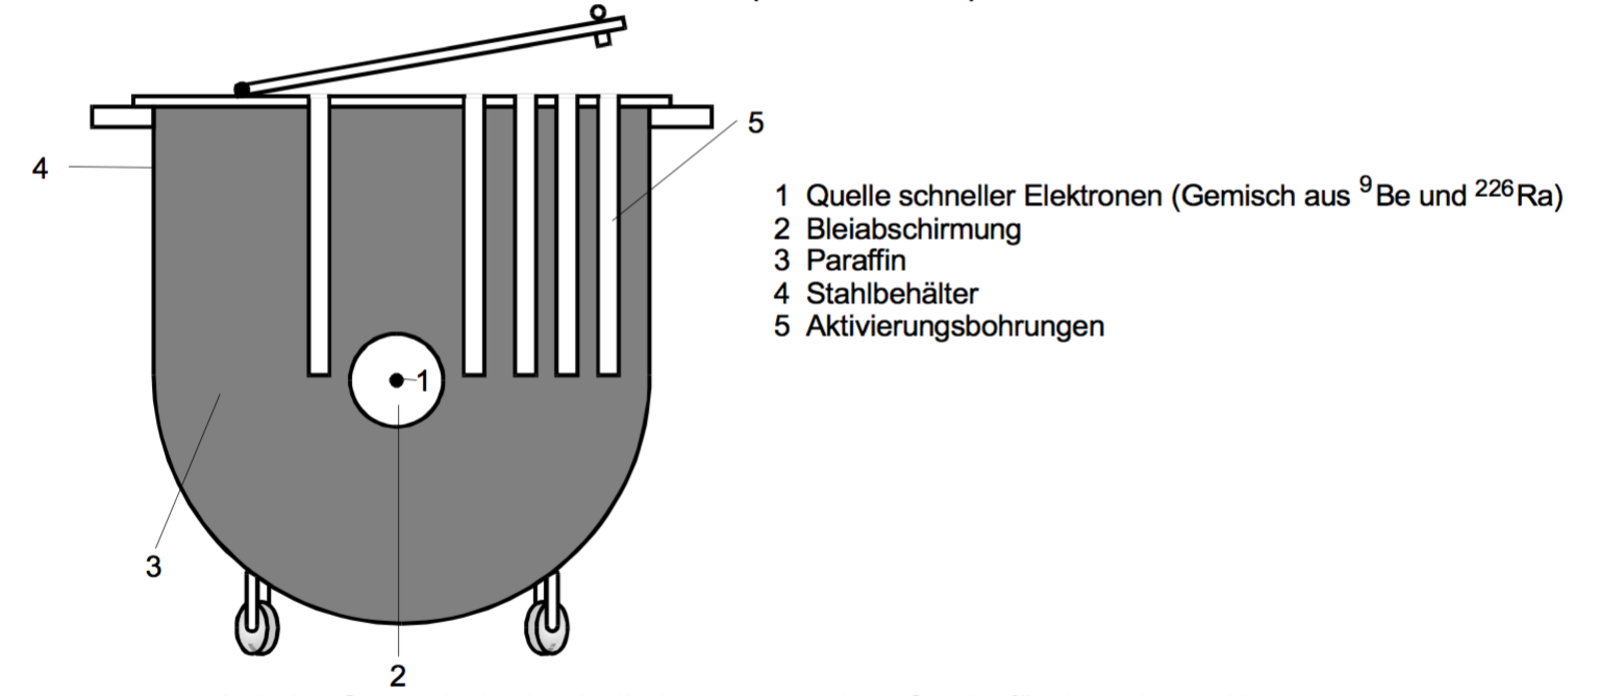
\includegraphics[width = \textwidth]{Pics/aktivierungsbehaelter.pdf}
  \caption{Behälter zur Aktivierung mit Neutronen.\cite{anleitung}}
  \label{fig:aktivierung}
\end{figure}

%Figureaktivierung

\subsection{Untersuchung des Zerfalls instabiler Isotope}

Im folgenden Versuch werden Jod und Rhodium aktiviert und dann die Halbwertszeit
der instabilen Isotope untersucht. Der Verlauf ist an folgenden Gleichungen
gezeigt:
\begin{align}
  \ce{^127_53 J + n&-> ^128_53 J -> ^128_54 XE + \beta^- + \bar{\g{\nu}_e}}\\
  \ce{^103_45Rh + n&}
  \begin{cases}
    \underrightarrow{\SI{10}{\percent}} \ce{^{104i}_45Rh -> ^104_45Rh &+ \text{$\gamma$} -> ^104_46Pd + \beta^- + \bar{\g{\nu}_e}}\\
    \underrightarrow{\SI{90}{\percent}} \ce{^104_45Rh -> ^104_46Pd &+ \beta^- + \bar{\g{\nu}_e}}.
  \end{cases}\label{eqn:zerfrho}
\end{align}

Während des radioaktiven Zerfalls nimmt die Anzahl instabiler Kerne nach
Formel \eqref{eqn:zerfall} ab.
\begin{equation}
  N(t) = N_0 e^{-\lambda t}
  \label{eqn:zerfall}
\end{equation}
$N_0$ ist die zu Beginn vorhandene Anzahl und $\lambda$ ist die Zerfallskonstante.
Über
\begin{align}
  \frac{1}{2} N_0 &= N_0 e^{-\lambda T}\\
  \intertext{folgt für die Halbwertszeit}
  T &= \frac{ln(2)}{\lambda}.
  \label{eqn:HalbwertszeitSteigung}
\end{align}

Die Halbwertszeit wird hier aber nicht aus $N(t)$ bestimmt, sondern es wird immer
$N_{\Delta t}(t)$ in einem festen Zeitintervall $\Delta t$ bestimmt.
Beschrieben wird $N_{\Delta t}(t)$ durch Formel \eqref{eqn:ndelta}.
\begin{align}
  N_{\Delta t}(t) &= N_0(1 - e^{-\lambda\Delta t}) e^{-\lambda t} \label{eqn:ndelta}\\
  \intertext{linearisiert ergibt sich so:}
  ln(N_{\Delta t}(t)) &= ln\left( N_0(1-e^{-\lambda\Delta t}\right) - \lambda t \label{eqn:ndeltalinear}.
\end{align}
Das $\Delta t$ wurde in vorherigen Versuchen für jede Zerfallsreihe bestimmt und kann hier übernommen
werden. Mit diesem Wissen kann die Halbwertszeit für Jod und andere Isotope bestimmt werden,
die nur eine unverzweigte Zerfallsreihe aufweisen.
Bei Rhodium liegt ein komplizierterer Sachverhalt vor. Nach der Aktivirerung kommen
wie in Formel \eqref{eqn:zerfrho} zwei Zerfallsreihen vor, die unterschiedliche Halbwertszeiten
haben. Da die $\gamma$-Emission bei der oberen Zerfallsreihe ebenfalls detektiert wird,
werden die Zerfälle ungefähr im gleichen Verhältnis aufgenommen.

Die beiden Zerfälle überlagern sich dann. Die Zerfallsreihe mit kürzerer Halbwertszeit
ist ab einem Zeitpunkt $t^*$ nicht mehr relevant und die langsame Zerfallsreihe bestimmt den restlichen Verlauf
der additiven Kurve. In Abbildung \ref{fig:additivekurve} ist diese Kurve eingezeichnet.%Figure additive Kurve
\begin{figure}[h]
  \centering
  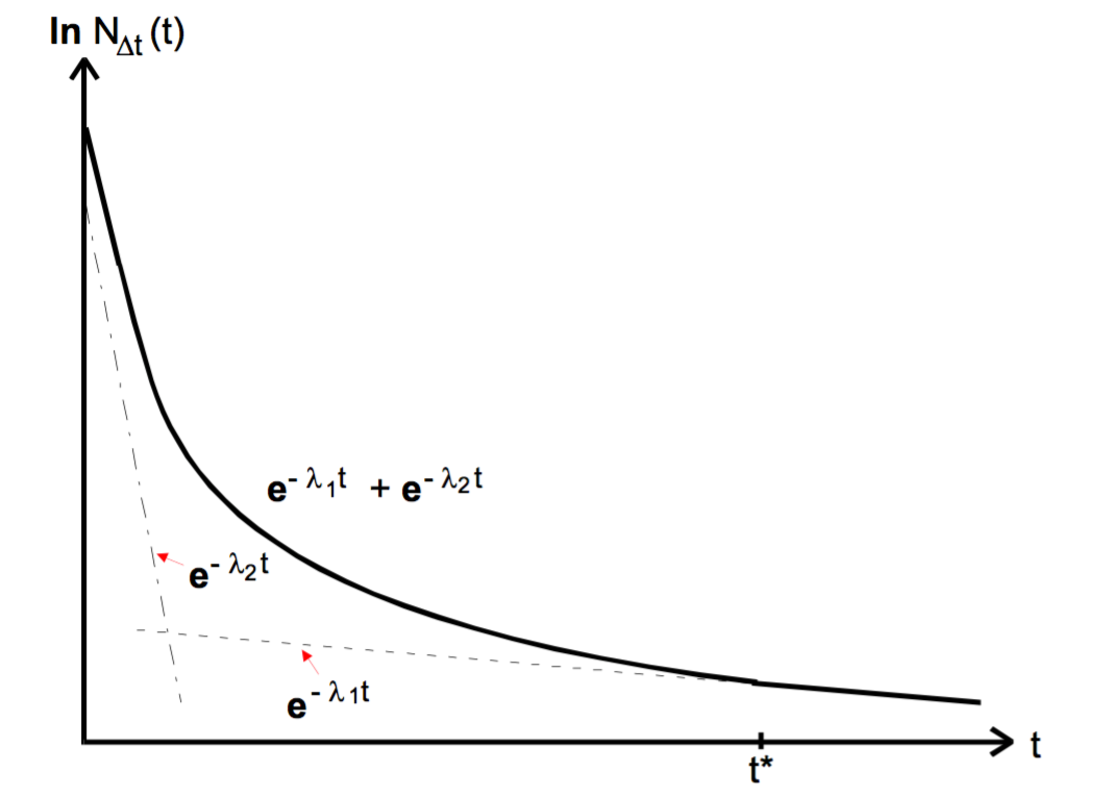
\includegraphics[width = \textwidth]{Pics/additivekurve.pdf}
  \caption{Zerfallskurve eines aus 2 Isotopen mit unterschiedlichen Zerfallskonstanten
   ($\lambda_2 << \lambda_1$) bestehenden Präparats.\cite{anleitung}}
  \label{fig:additivekurve}
\end{figure}
Dann kann der Verlauf der langsamen Kurve bestimmt werden und durch Subtraktion
von der kurzlebigen Kurve für beide Zerfälle die Halbwertszeit bestimmt werden.
